\documentclass[a4paper]{amsart}
\usepackage{units}
\usepackage{multirow}
\usepackage{amstext}
\usepackage{amsmath}
\usepackage{amssymb}
\usepackage{amsfonts}
\usepackage{enumerate}
\usepackage{cite}
%\usepackage{natbib}
\usepackage{amsthm}
\usepackage{array,arydshln}
\usepackage[pdftex]{graphicx}
\usepackage{rotating}
\usepackage{ifpdf}
%\usepackage{epsfig}
\usepackage[all]{xy}
\usepackage{latexsym}
\usepackage[hidelinks]{hyperref}
\usepackage{color}
\usepackage{wrapfig}
\usepackage{caption}
\usepackage{blkarray}
\usepackage{array}


\makeatletter
%%%%%%%%%%%%%%%%%%%%%%%%%%%%%% Textclass specific LaTeX commands.
\numberwithin{equation}{section} %% Comment out for sequentially-numbered
\numberwithin{figure}{section} %% Comment out for sequentially-numbered
\numberwithin{table}{section}
\let\footnote=\endnote
\theoremstyle{plain}
\newtheorem{thm}{Theorem}[section]
\theoremstyle{definition}
\newtheorem{defn}[thm]{Definition}
\newtheorem{Def}[thm]{Definition}
\newtheorem{definition}[thm]{Definition}
\newtheorem{exam}[thm]{Example}
\newtheorem{example}[thm]{Example}
\newtheorem{algo}[thm]{Algorithm}
\newtheorem{note}[thm]{Note}
\theoremstyle{plain}
\newtheorem{assumption}[thm]{Assumption}
\theoremstyle{plain}
\newtheorem{lem}[thm]{Lemma}
\newtheorem{lemma}[thm]{Lemma}
\theoremstyle{plain}
\newtheorem{cor}[thm]{Corollary}
\newtheorem{corollary}[thm]{Corollary}
\theoremstyle{plain}
\newtheorem{rmk}[thm]{Remark}
\newtheorem{rem}[thm]{Remark}
\theoremstyle{plain}
\newtheorem{Proposition}[thm]{Proposition}
\newtheorem{pro}[thm]{Proposition}


%\newcommand{\norm}[1]{\|#1\|}
\def\norm#1{\|#1\|}
\def\normm#1#2{\|#1\|_{#2}}
\def\normF#1{\|#1\|_{F}}
\def\Proof{{\bf Proof.\enspace}}
\def\vec{\mathrm{vec}}
%\def\unvec{\mathrm{unvec}}
\def\tr{\mathrm{tr}}
%\def\tr{\textrm{tr}}
\def\bmatrix#1{\left[\begin{matrix}#1\end{matrix}\right]}
\def\pmatrix#1{\left(\begin{matrix}#1\end{matrix}\right)}
\def\R{\mathbb{R}}
\def\N{\mathbb{N}}
\def\C{\mathbb{C}}
\def\nbyn{n\times n}
\def\mbyn{m\times n}
\def\mbym{m\times m}
\def\pbyq{p\times q}
\def\nnbynn{n^{2}\times n^{2}}
\def\mbf#1{\mathbf{#1}}
\def\mrm#1{\mathrm{#1}}
\def\bpi{\boldsymbol{\pi}}
\def\a{\alpha}
\def\b{\beta}
\def\d{\delta}
\def\e{\varepsilon}
\def\l{\lambda}
\def\D{\mathcal{D}}
\def\F{\mathcal{F}}
\def\G{\mathcal{G}}
\def\Q{\mathcal{Q}}
\def\M{\mathcal{M}}
\def\P{\mathcal{P}}
\def\dpm#1{\begin{displaymath}#1\end{displaymath}}
\def\bdm{\begin{displaymath}}
\def\edm{\end{displaymath}}
\def\beq{\begin{equation}}
\def\eeq{\end{equation}}
\def\dtyl{\displaystyle}
\def\ones#1{\mathbf{1}_{#1}}
%\def\onesn{\mathbf{1}_{n \times n}}

\makeatother

\title[Development of an Algorithm Improving Label Arrangements]{Development of an Algorithm Improving Label Arrangements in Offset Printing}

%\authorrunning{Short form of author list} % if too long for running head

\author[G. S. Jang]{Geun Soo Jang}
\address{Geun Soo Jang\\
	Finance.Fishery.Manufacture Industrial Mathematics Center on Big Data, Pusan National University, Busan, 46241, Republic of Korea}
\email{sand621@naver.com}
\author[T. H. Kim]{Taehyeong Kim}
\address{Taehyeong Kim\\
	Finance.Fishery.Manufacture Industrial Mathematics Center on Big Data, Pusan National University, Busan, 46241, Republic of Korea}
\email{xogud7936@pusan.ac.kr}
\author[H.-M. Kim]{Hyun-Min Kim}
\address{Hyun-Min Kim\\
	Finance.Fishery.Manufacture Industrial Mathematics Center on Big Data, Pusan National University, Busan, 46241, Republic of Korea}
\email{hyunmin@pusan.ac.kr}
\author[K. M. Kong]{Ki Man Kong}
\address{Ki Man Kong\\
	World Komax Co., Ltd., 1505, Centum Jungang-Ro 48,Haeundae-Gu, Busan, 48059, Republic of Korea}
\email{kennethkong@worldkomax.net}
\author[J. R. Park]{Jeong Rye Park}
\address{Jeong Rye Park\\
	Finance.Fishery.Manufacture Industrial Mathematics Center on Big Data, Pusan National University, Busan, 46241, Republic of Korea}
\email{parkjr@pusan.ac.kr}
\author[J.-H. Seo]{Jong-hyeon Seo}
\address{Jong-hyeon Seo\\
	Chubu University Academy of Emerging Science, Kasugai, 487-0027, Japan}
\email{hyeonni94@gmail.com}
\author[S.-H. Seo]{Sang-hyup Seo$^{\dagger}$}
\address{Sang-hyup Seo\\
	Finance.Fishery.Manufacture Industrial Mathematics Center on Big Data, Pusan National University, Busan, 46241, Republic of Korea}
\email{saibie1677@gmail.com}
\author[S. W. Yoon]{Shin won Yoon}
\address{Shin won Yoon\\
	Finance.Fishery.Manufacture Industrial Mathematics Center on Big Data, Pusan National University, Busan, 46241, Republic of Korea}
\email{ysw0123@pusan.ac.kr}
\thanks{$^{\dagger}$Corresponding author}
%\markleft{G. S. Jang, T. H. Kim, H.-M. Kim, K. M. Kong, J. R. Park, J.-H. Seo, S.-H. Seo, S. W. Yoon}
%\date{Received: date / Accepted: date}
% The correct dates will be entered by the editor

\begin{document}

\begin{abstract}
One of the most classic problems in the manufacturing industry is inventory processing. 
There is a way to effectively reduce inventory by 
changing the array of the pieces on the printing plates in the offset printing. 
It is setting an upper limit of acceptable for each plate, and carrying out complete enumeration. 
This method dramatically reduces the operating time of the algorithm. 
The advantage of this method is that it focuses on changing the arrangement of the pieces on the plates.
\end{abstract}
\subjclass[2010]{68U99, 90C90}
\keywords{Offset Printings \and Combinations with Repetition \and Label Arrangements \and Inventory Managements}

\maketitle

\markleft{G. S. Jang, T. H. Kim, H.-M. Kim, K. M. Kong, J. R. Park, J.-H. Seo, S.-H. Seo, and S. W. Yoon}

\section{Introduction}\label{sec:intro}
A combination with repetition is the number of cases, where $k$ elements are selected from among different $n$ elements allowing repetition \cite{Brualdi2004}. 
It is indicated with the symbol $_{n}H_{k}$ and the following is established.
\begin{equation}
	_{n}H_{k} = _{n+k-1}C_{k} = \frac{(n+k-1)!}{(n-1)!k!}
\end{equation}
For instance, the combination with repetition $_{2}H_{4}$ to select four elements from among two elements A and B comprises the following five cases.
\begin{enumerate}[(1)]
	\item $\textrm{[A, A, A, A]}$ : a list consisting of four A's
	\item $\textrm{[A, A, A, B]}$ : a list consisting of three A's and one B
	\item $\textrm{[A, A, B, B]}$ : a list consisting of two each of A's and B's
	\item $\textrm{[A, B, B, B]}$ : a list consisting of one A and three B's
	\item $\textrm{[B, B, B, B]}$ : a list consisting of four B's
\end{enumerate}
Among the above cases, if we want to obtain three A's and nine B's, then we can choose $[\textrm{A, B, B, B}] \times 3$. 
Also, we consider the following as another case.
\begin{equation}\label{eq:3lists}
	\textrm{[A, A, B, B]} \times 1 + \textrm{[A, B, B, B]} \times 1 + \textrm{[B, B, B, B]} \times 1
\end{equation}
In this case, we can get the three A's and nine B's. 
However, the former case seems to be a ‘Better’ because there are three different lists in (\ref{eq:3lists}). 
Let us examine the other case.
\begin{equation}
\textrm{[A, A, A, A]} \times 1 + \textrm{[B, B, B, B]} \times 3 - \textrm{[A]} \times 1 - \textrm{[B]} \times 3
\end{equation}
$\textrm{[A, B, B, B]} \times 3$ also seems to be `Better' because there is no loss. Under the following conditions, $\textrm{[A, B, B, B]} \times 3$ is the ‘Best’ method.
\begin{enumerate}[(1)]
	\item Minimize the number of list.
	\item Minimize the loss of lists.
\end{enumerate}
Offset printing, also called offset lithography, or litho-offset, in commercial printing, 
widely used printing technique in which the inked image on a printing plate is printed on a rubber cylinder and then transferred (i.e., offset) to paper or other material. 
The rubber cylinder gives great flexibility, permitting printing on wood, cloth, metal, leather, and rough paper (see Figure \ref{fig:OffsetPrint}) \cite{OffsetPrint}.

\begin{figure}[h!]
	\centering
	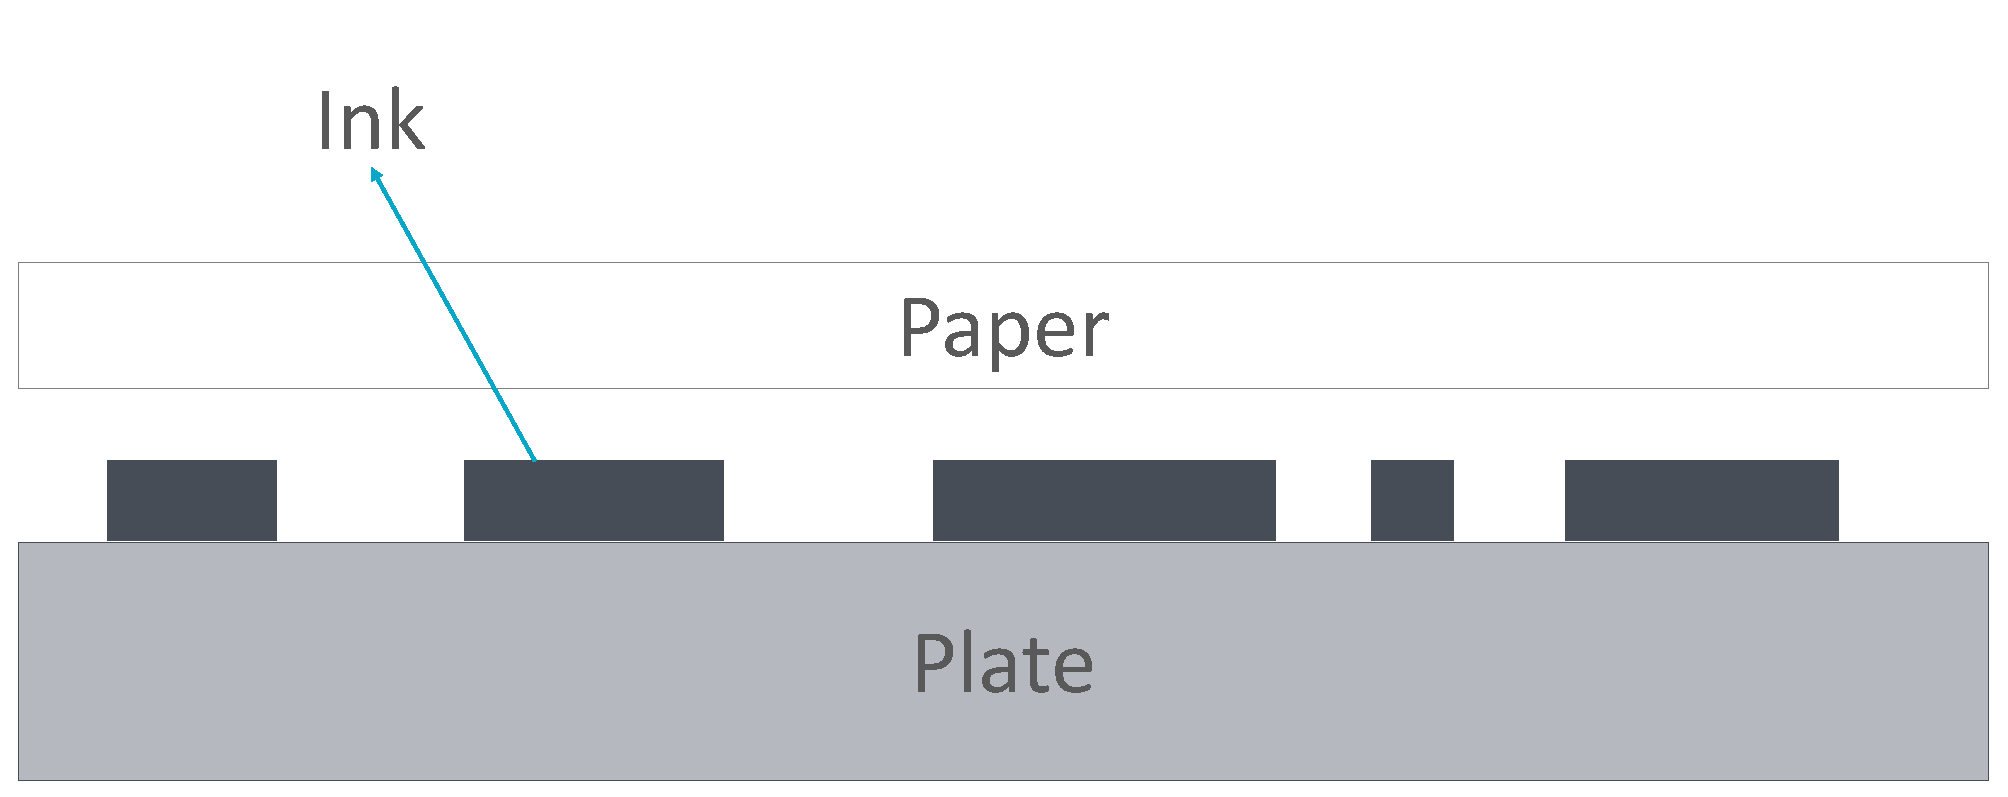
\includegraphics[width=7cm]{OffsetPrint.pdf}
	\caption{Offset Printing}
	\label{fig:OffsetPrint}
\end{figure}

Offset printing is one of the most common ways of creating printed materials. A few of its common applications include: newspapers, magazines, brochures, stationery, and books. Compared to other printing methods, offset printing is best suited for economically producing large volumes of high quality prints in a manner that requires little maintenance \cite{Kipphan2001}. 
To improve printing process, there were many researches in \cite{AlChan, Muscle, Carmo}.
As an other improving, how to make the initial plates is an important issue. Above example means that what is the best arrangement in such print method.

In the past, production was based on ordering of products from companies and predictions of consumption. 
However, as the internet market has became popular, the production systems have been changed by consumers. 
Now, many factories produce only products ordered by consumers.

World Komax is a company that produces labels using the offset printing. The labels refer to stickers containing bar-codes attached to garments or shoes as follows (see Figure \ref{fig:AirHuarache}). Each bar-code in the label contains fixed information such as product names and colors, and variable information such as the date of manufacture.

\begin{figure}[h!]
	\centering
	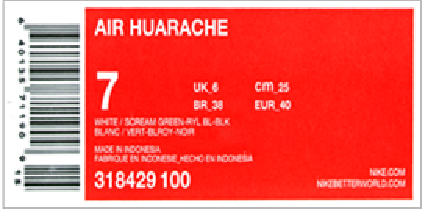
\includegraphics[width=6.5cm]{AirHuarache.pdf}
	\caption{Sneaker Review : Nike Air Huarache}
	\label{fig:AirHuarache}       % Give a unique label
\end{figure}

\noindent
Since the program of World Komax is not suitable for small quantity batch productions, the number of labels loss increased compared to the past.

Section 2 of this paper will describe the process of label printing using offsets. The modeling of the problem will be carried out in Section 3, and examples to help the understanding of the problem will be prepared in Section 4. The final results of the algorithm will be described in Section 5. 


\section{Offset label printing process}\label{sec:Offset}

\subsection{Label printing process}\label{subsec:LabelPrinting}
Before discussing the process of label printing, we define the following terms.
\begin{enumerate}[*]
	\item {\bf Plate} : A printing plate for the offset printing (see Figure \ref{fig:PlateLabel})
	\item {\bf Loss} : The number of labels printed in excess of the order-quantity
\end{enumerate}

The offset label printing process is as follows. At first, we receive orders from customers. The order includes many types of labels and order-quantities by type (see Figure \ref{fig:Order_Sorting}). Thereafter, offset printing plates are made. Many types of labels are placed on each plate so that many labels are printed at one printing. After the plates are made, we produce more labels than order-quantities using each plate. Then, the sheets are cut into the label size. As the final process, the labels are collected by type.

\begin{wrapfigure}{r}{4cm}
	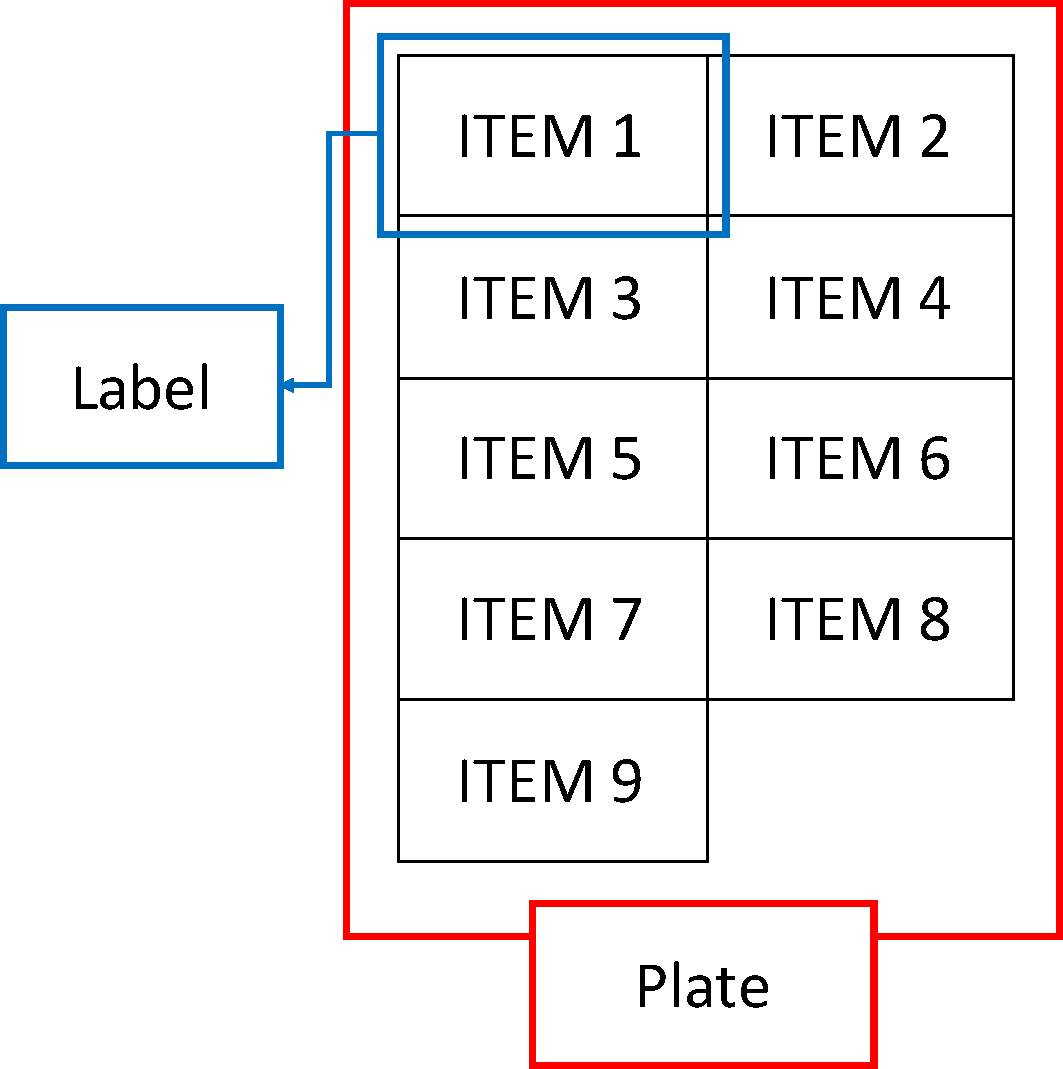
\includegraphics[width=4cm]{PlateLabel.pdf}
	\caption{Plate and Label}
	\label{fig:PlateLabel}       % Give a unique label
\end{wrapfigure}

\subsection{Major points for cost saving}\label{subsec:CostSave}
The constraint conditions and major points that will be considered in this paper for cost saving are as follows. First, one type of label should be placed on only one plate. This is to prevent different types of labels from being mixed when collected by type after the printed sheets are cut. Meanwhile, the total number of labels placed on each plate is also constant because the sizes of individual plates are constant and the sizes of labels in one order are also constant. In addition, the number of plates should be minimized as little as possible because plates are made using molds and the costs are high. Finally, the Loss should be minimized because overprinted labels cannot be used and should be entirely discarded.

\subsection{Sorting reports output program}\label{subsec:SortProgram}
The production of plates and the use of printing paper incur costs. To reduce the costs, order details are inputted to output appropriate methods to place labels on the plate as sorting reports. The plate makers produce plates according to the instructions in the sorting reports (see Figure \ref{fig:Order_Sorting}).

Since the existing sorting report output method was not suitable for small quantity batch production systems, the algorithm should be improved. Therefore, this study was conducted to develop new algorithms suitable for small quantity batch production systems too.

\begin{figure}[h!]
	\centering
	\resizebox{14cm}{7cm}{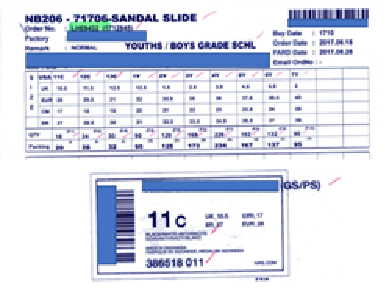
\includegraphics{OrderForm.pdf}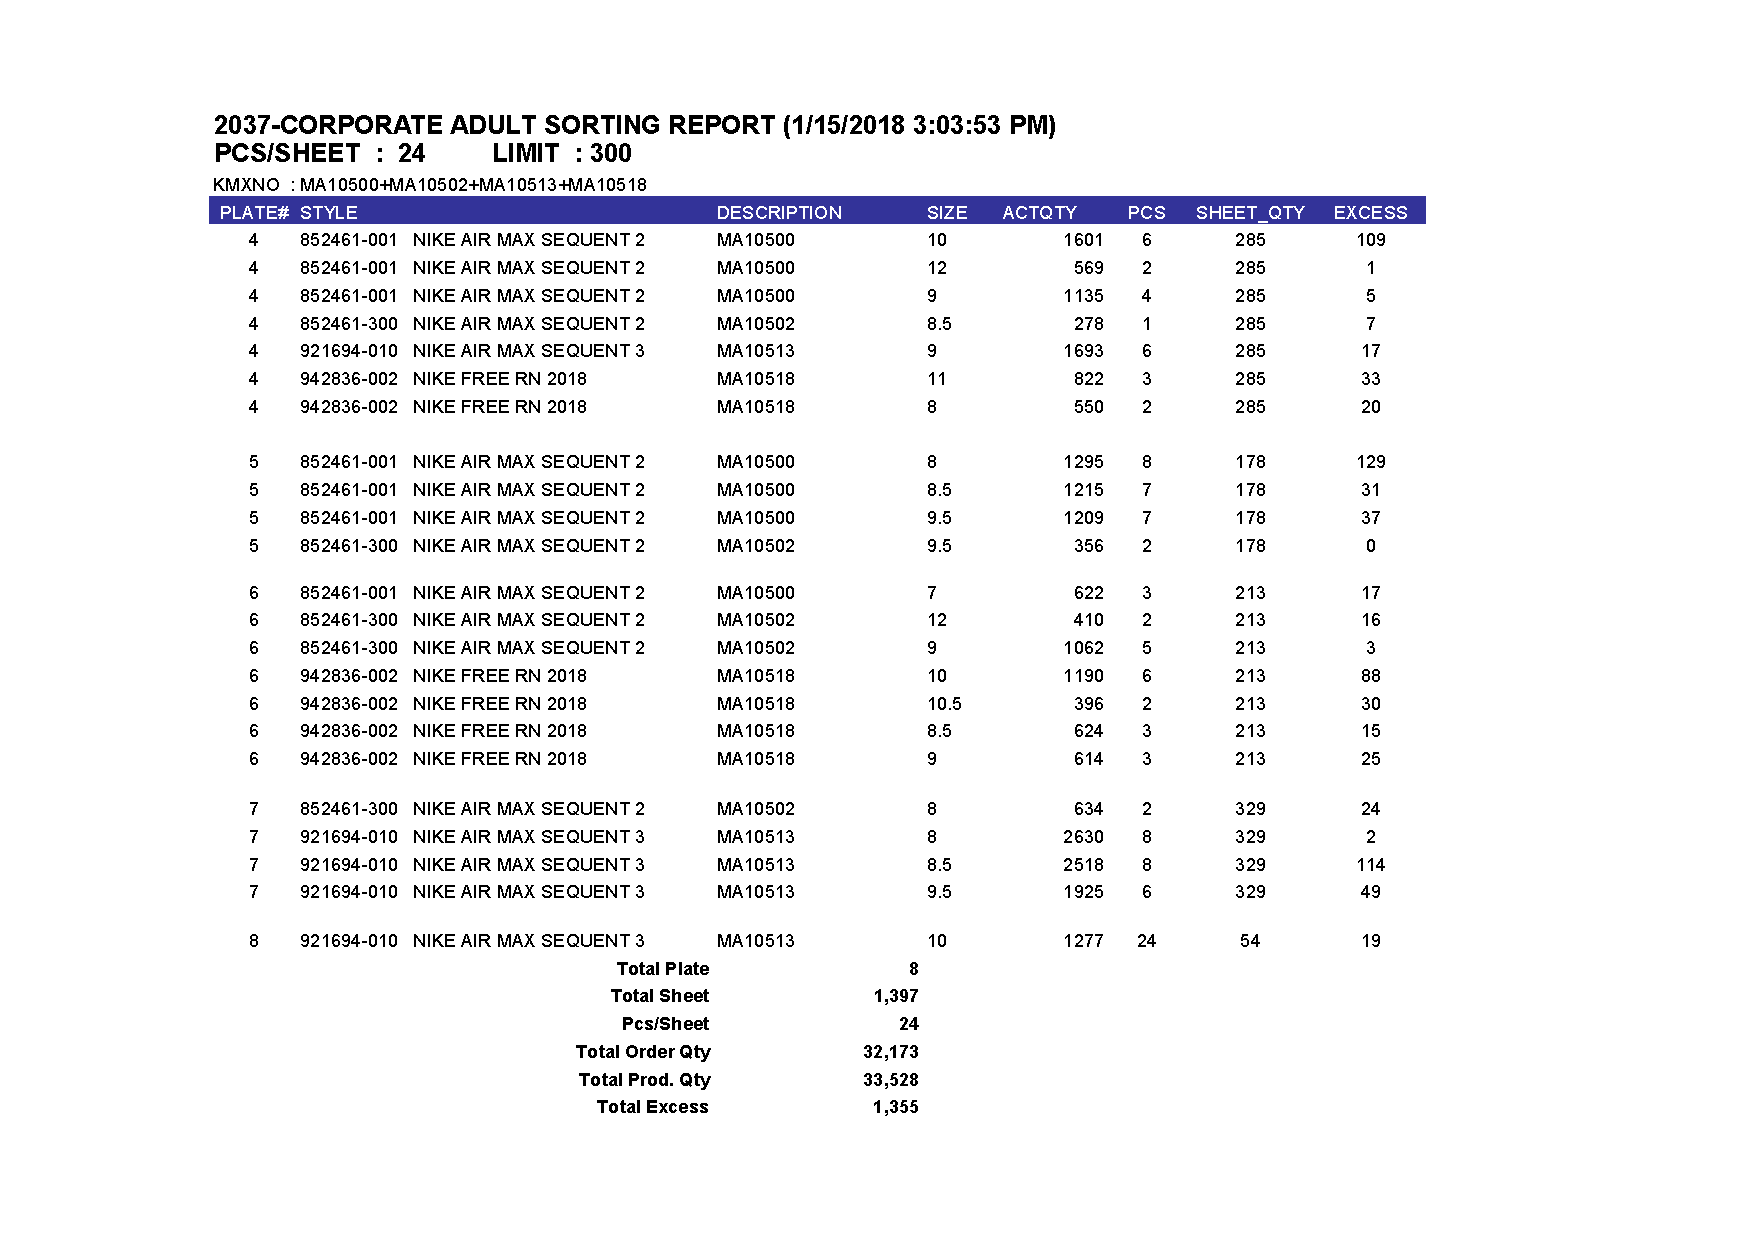
\includegraphics{SortingReport.pdf}}\\
	\caption{An Order Form(left) and a Sorting Report(right) \\(Source: World Komax Co., Ltd.)}
	\label{fig:Order_Sorting}       % Give a unique label
\end{figure}

\section{Modeling and flowchart}\label{sec:Modeling}
To formulate our problem as a mathematical optimization problem, we first need to define our notation.
\begin{enumerate}[$\bullet$]
	\item Let $I$ be a set of products.
	\item For each product $i \in I$, let $b_{i}$ be the number of order.
	\item Let ${\bf b}=(b_{i}|i \in I)$ be a vector of order-quantities.
	\item $k$ is the total number of labels that can be placed in one Plate.
	\item $\pi$ is a partition of $I$ such that $1 \leq  |P| \leq k$ for any $P \in \pi$. 
	\item Let $\Gamma_{\pi}$ be a set of matrix $A \in {\rm Mat}_{\pi \times I}(\mathbf{Z})$ satisfy the following:
	\begin{itemize}
		\item[-] For all $(P,i) \in \pi \times I$, $A_{P,i} \geq 0$, and $A_{P,i} = 0$ if and only if $i \notin P$.
		\item[-] For each $P \in \pi$, $\sum_{i \in P}A_{P, i} = k$
\end{itemize}
\end{enumerate}

Using the above notation,
\begin{equation}\label{eq:NumPlate}
	\left\lceil \max \left\{ \left.\frac{b_{i}}{A_{P,i}}\right|i \in P \right\} \right\rceil
\end{equation}
is the printing number of Plate $P$, where $\lceil~\rceil$ means the ceiling. 
Assume that $\alpha$ is the cost to produce one Plate, and $\beta$ is the cost of the loss of one label. 
Then, our goals is to obtain the following 
\begin{equation}\label{eq:TotalCost}
	\min_{\pi} \{ \alpha|\pi| + \beta E_{A,b} | A \in \Gamma_{\pi} \}
\end{equation}
where
\begin{equation}\label{eq:TotalLoss}
	E_{A,b} = \sum_{P \in \pi} \sum_{i \in I} \left( \left\lceil \max \left\{ \left.\frac{b_{i}}{A_{P,i}}\right|i \in P \right\} \right\rceil \cdot A_{P,i} - b_{i} \right)
\end{equation}
means the total number of losses of labels.

Naturally, the complete enumeration using combinations with repetition is the surest way. 
However, this method has a problem that it takes too much time. 
For instance, when $n=65$ and $k = 24$, the combination with repetition $_{65}H_{24}$ comprises about $2.36 \times 10^{21}$ cases.
Then, the calculation of the cases takes more than 658 hours, that is, more than 27 days using a super computer that can calculate $10^{15}$ partitions per second. 
Given that there are limits of the time from the date of receipt of orders to the delivery date, this is a very long computation time.

In this algorithm, this problem was solved by introducing any positive integers as thresholds. 
Thresholds mean the allowed amount of losses occurring in each plate. 
Adopting a partition that does not exceed the threshold will dramatically reduce the time taken.
Based on the foregoing, the flowchart of the algorithm can be set forth as follows (see Figure \ref{fig:MFChart}).

\begin{figure}[h!]
	\centering
	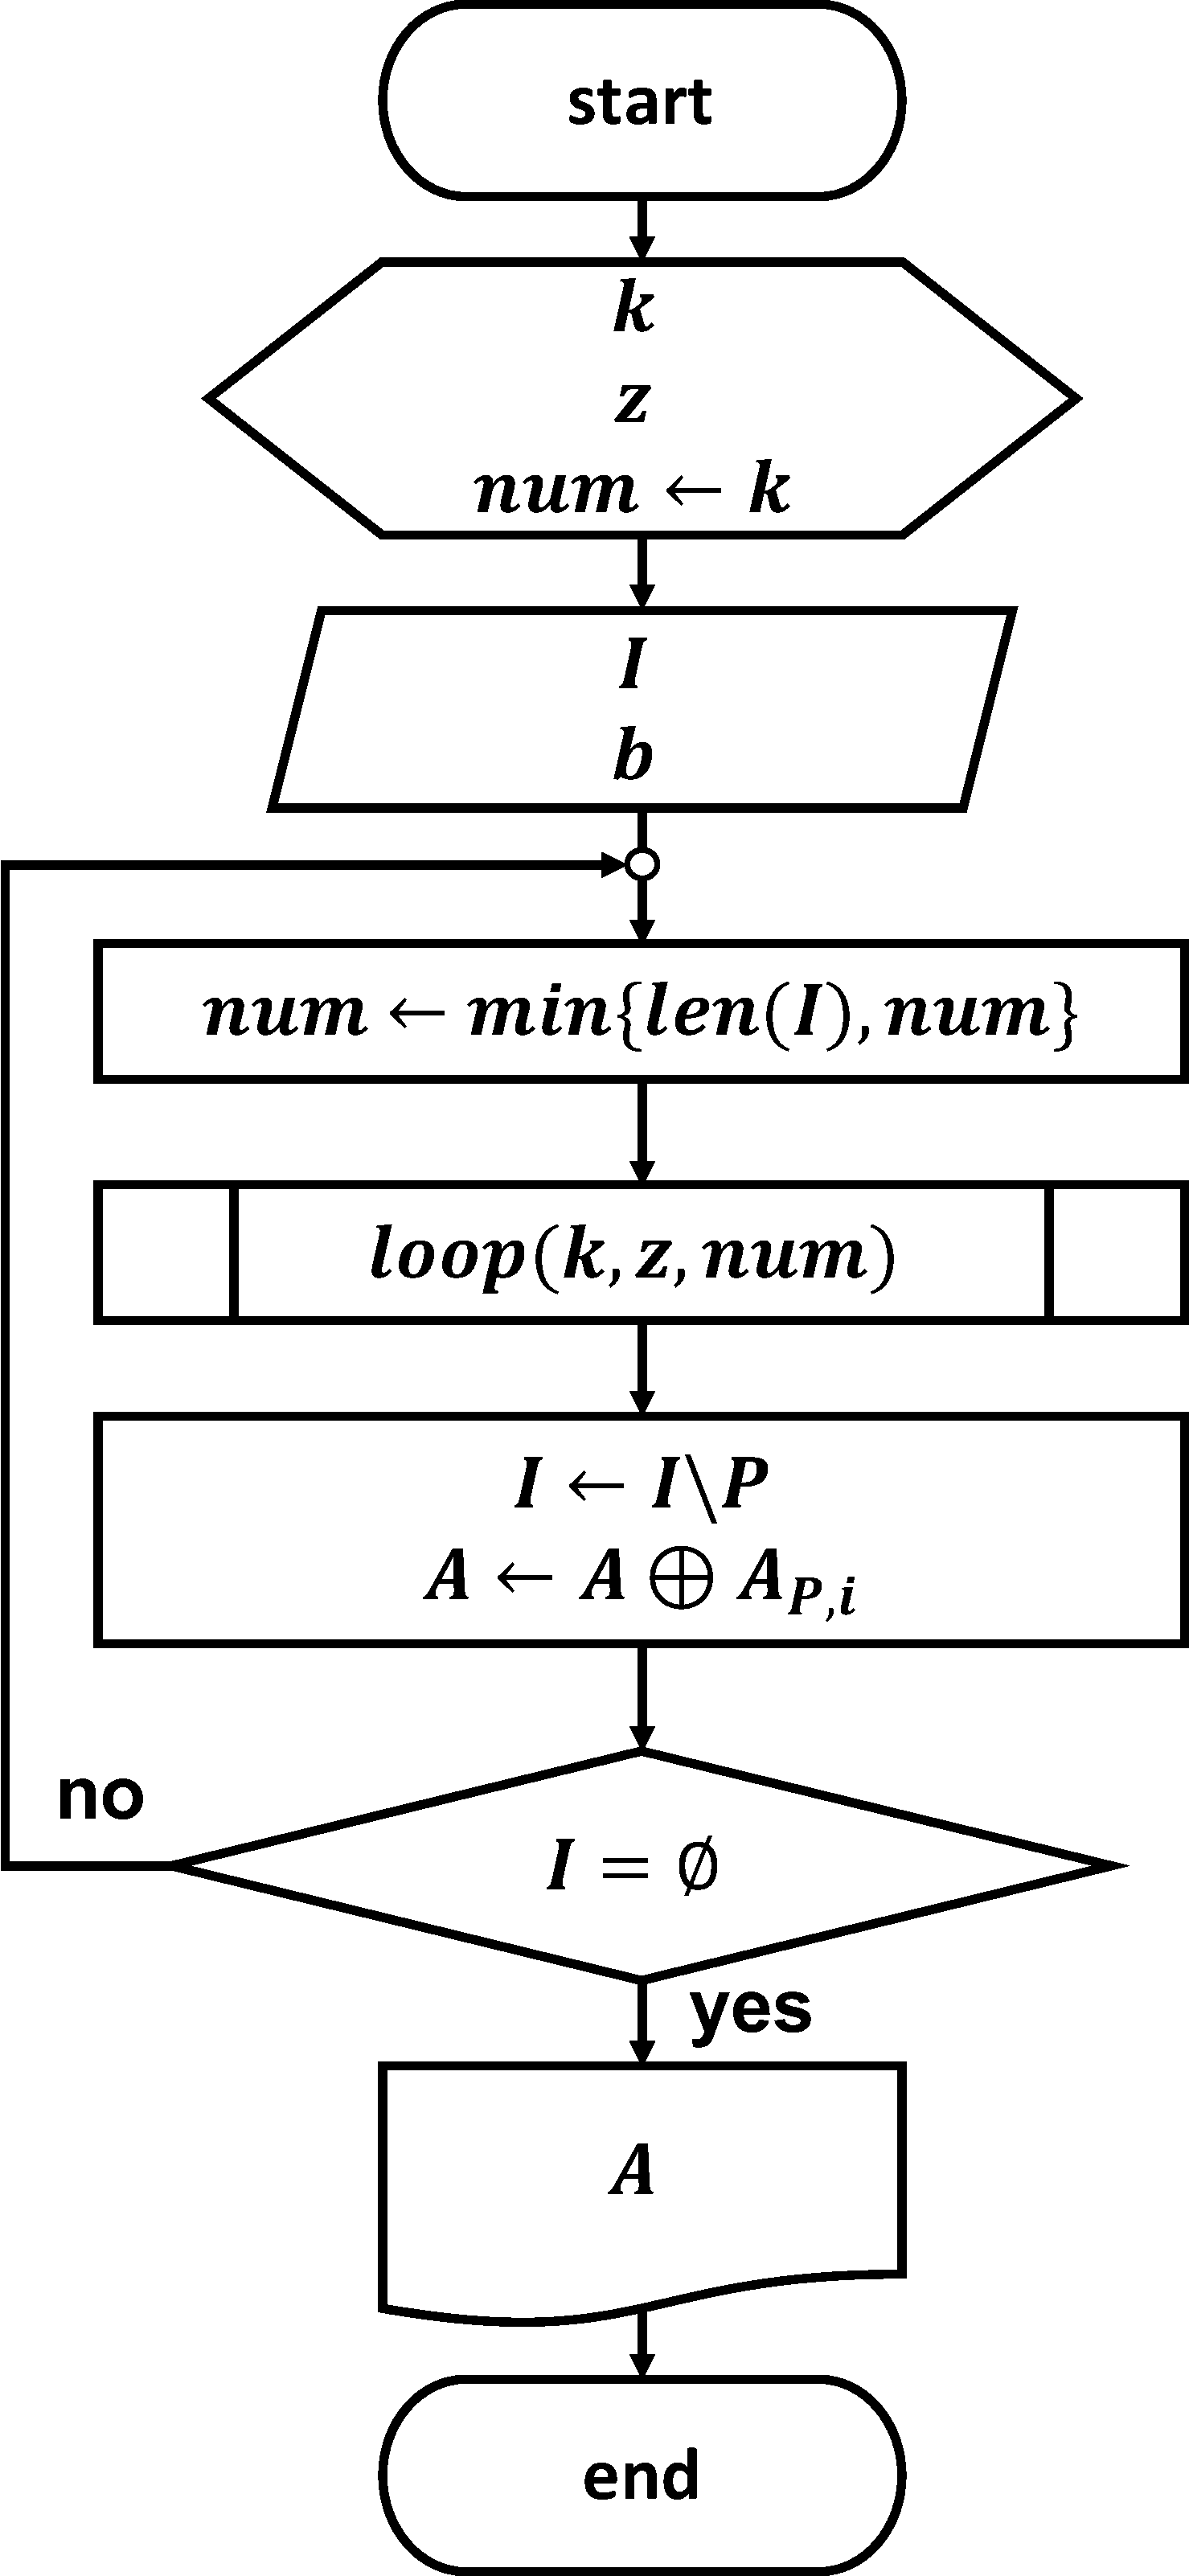
\includegraphics[width=4cm]{MainFChart.pdf}
	\caption{The Main Flowchart}
	\label{fig:MFChart}       % Give a unique label
\end{figure}

In Figure \ref{fig:MFChart}, $z$ is the threshold and the others are explained in the notation above.
This algorithm outputs matrix $A=\bigoplus\limits_{P} A_{P,i}$ containing the label of each product when $I$ and ${\bf b}$ have been inputted for $z$, $k$, $num$. 
One of the results of ${loop}(k, z, num)$, $P$ is the products that contain the Plate (see Figure \ref{fig:SFChart}). 
By removing $P$ from $I$, each plate does not have the same product.
The algorithm repeats until $I$ is empty.

\begin{figure}[h!]
	\centering
	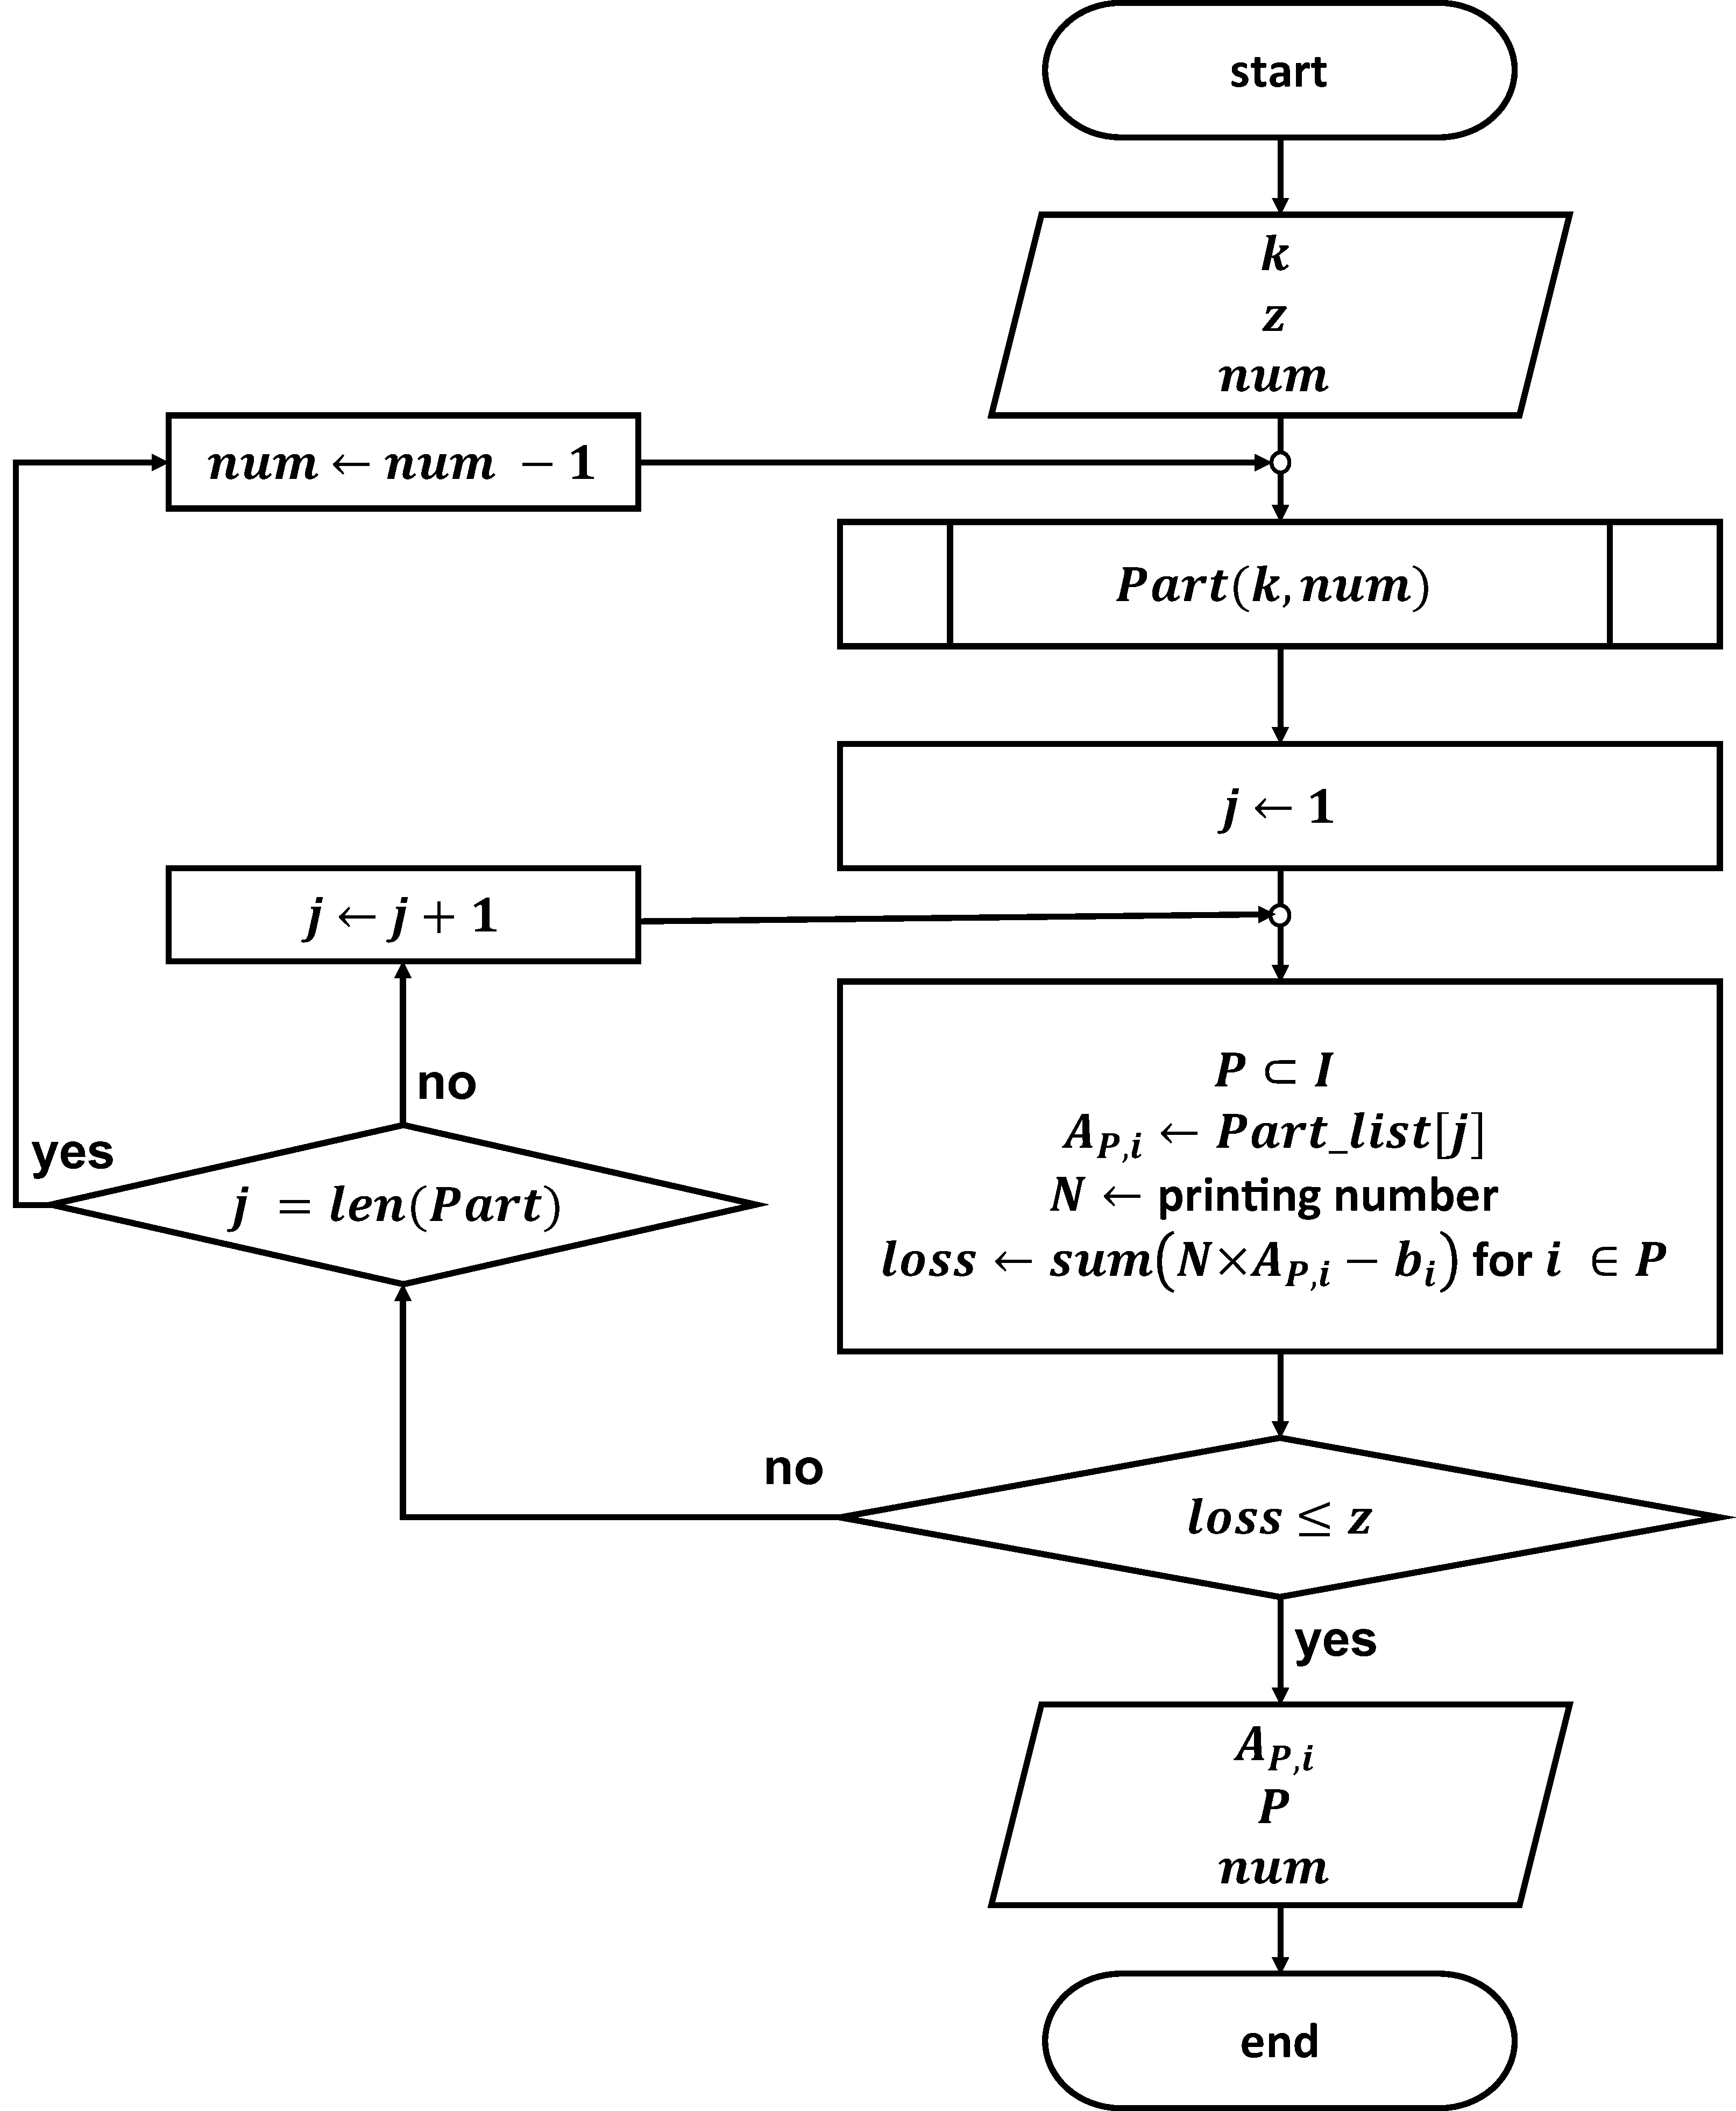
\includegraphics[width=8cm]{SubFChart.pdf}
	\caption{The Flowchart of ${loop}(k, z, num)$}
	\label{fig:SFChart}       % Give a unique label
\end{figure}

Meanwhile, in the case of the ${loop}(k, z, num)$ function, the flowchart in Figure \ref{fig:SFChart} should be followed.
First, the ${Part}(k, num)$ function finds partitions using the combination with repetition $_{num}H_{k}$ 
%(method to select $k$ pieces of products from $num$ pieces of products allowing repetition)
and indicated in the form of a list. 
We set the result as {\it Part\underline{ }list}.
For example, let $k=6$ and $num=3$, then $\text{\it Part\underline{ }list}={Part}(6, 3) = \{ [4,1,1],[3,2,1],[2,2,2] \}$.
$N$ is a printing number that expressed in \eqref{eq:NumPlate}.
An appropriate $P$ that has $num$ pieces of products is selected from $I$ and the loss is obtained using {\it Part\underline{ }list} and the printing number.

If the loss exceeds the threshold $z$, another {\it Part\underline{ }list} will be selected and the foregoing will be repeated  while adjusting $num$ until the threshold $z$ is not exceeded.
As a result of this process, $A_{P,i}$ whose loss does not exceed the threshold is obtained.% (see Figure \ref{fig:SFChart}).



\section{Examples}\label{sec:Exam}
This example was described to help the understanding of the problem. For the next two examples, we assume that $k$ is equal to 4.

\begin{example}
	Assume that $I=\{1,2,3\}$, and ${\bf b}=(50,30,20)$.
	
	We consider $\pi = \{\{1,2\}, \{3\}\}$ is a partition for ${\bf b}$. 
	Without loss of generality, assume that $P_{1} = \{1,2\}, P_{2} = \{3\}$. Since $k = 4$, the matrix $A$ can be found as follows.
	
	\begin{equation}
		A = \left(\begin{array}{ccc}2 & 2 & 0 \\ 0 & 0 & 4 \end{array}\right)
	\end{equation}
	
	In this case, the printing numbers (\ref{eq:NumPlate}) of $P_1$ and $P_2$ are as follows, respectively.
	\begin{equation}
		\left\lceil \max\left\{ \left. \frac{b_{i}}{A_{P_{1},i}} \right| i \in P_{1} \right\} \right\rceil = \left\lceil \max \left\{ \frac{50}{2}, \frac{30}{2} \right\} \right\rceil = 25
	\end{equation}
	and
	\begin{equation}
	\left\lceil \max\left\{ \left. \frac{b_{i}}{A_{P_{2},i}} \right| i \in P_{2} \right\} \right\rceil = \left\lceil \max \left\{ \frac{20}{4} \right\} \right\rceil = 5.
	\end{equation}
	We can see the Figure \ref{fig:ex11} for more details.
	
	\begin{figure}[h!]
		\centering
		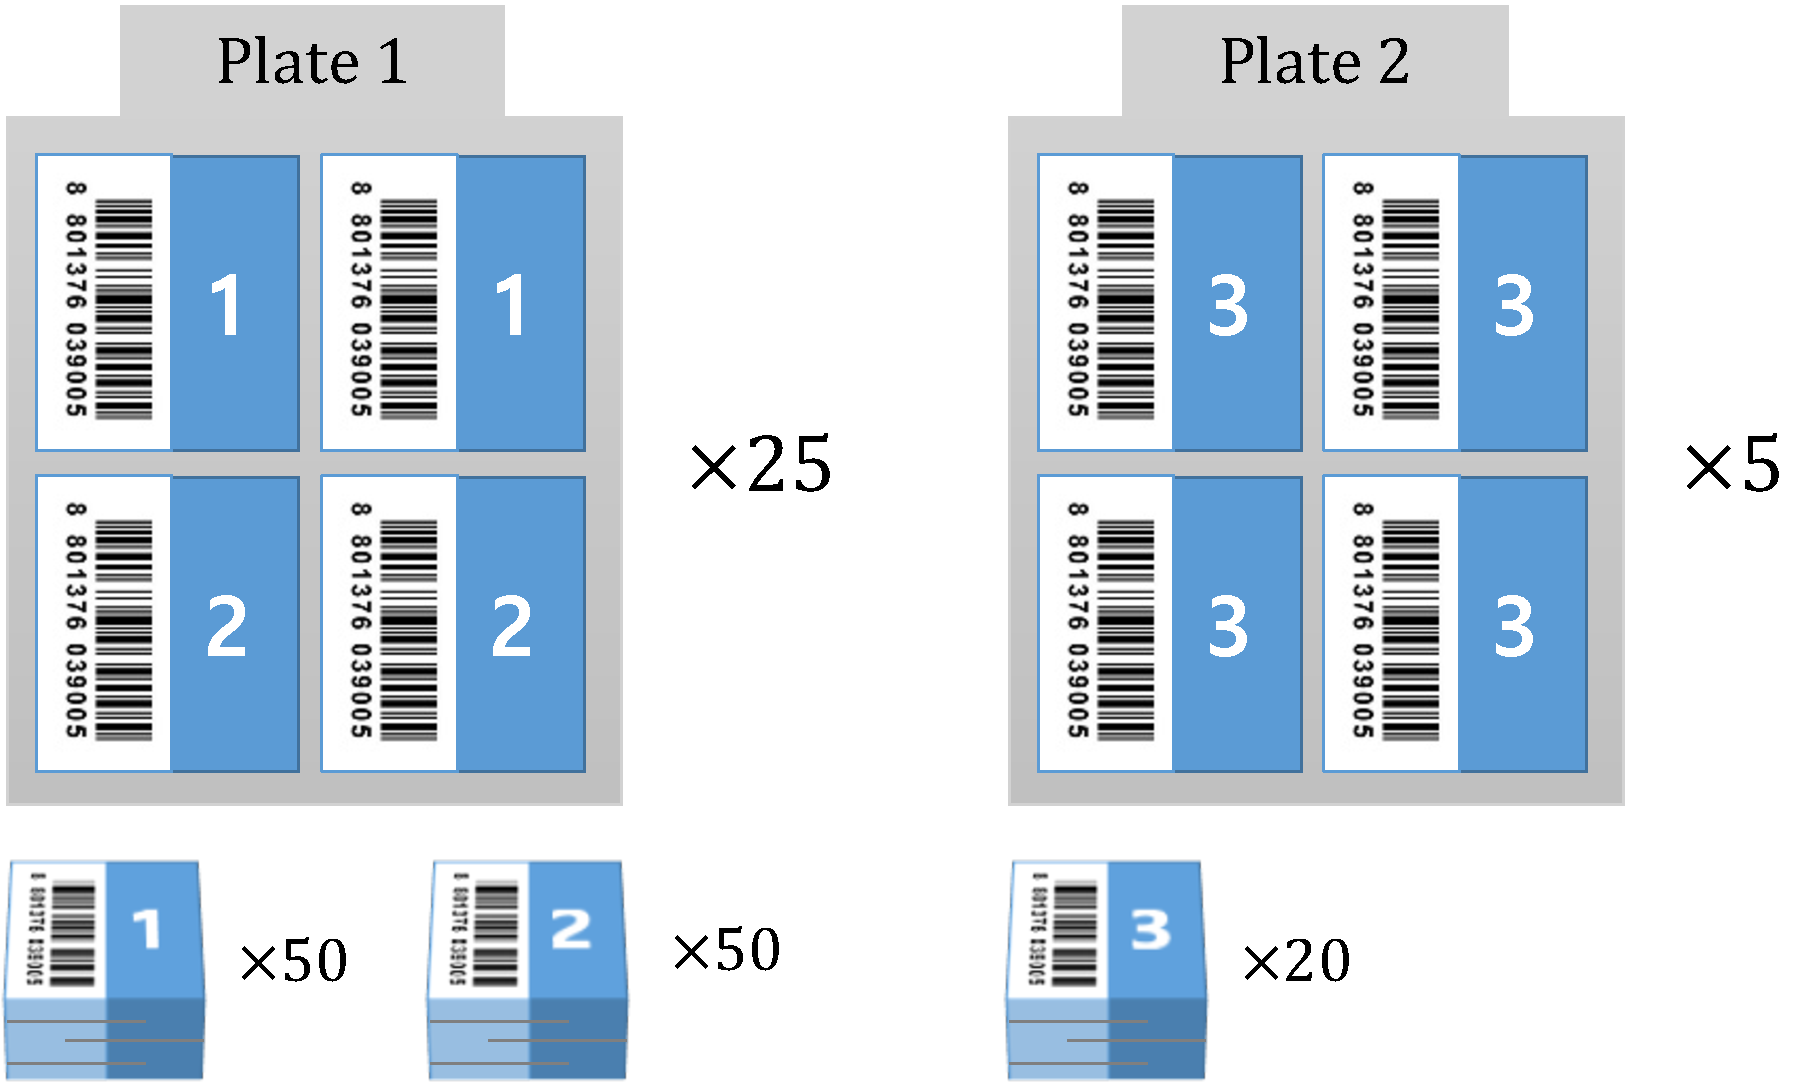
\includegraphics[width=6cm]{ex11.pdf}
		\caption{}
		\label{fig:ex11}       % Give a unique label
	\end{figure}
	
	It can be seen that the total number of Loss $E_{A,{\bf b}}$ is 20.
	
	Now, we consider a new partition $\pi = \{\{1,2,3\}\}$. In this case, $A = (\begin{array}{ccc}2 & 1 & 1 \end{array})$, and printing number (\ref{eq:NumPlate}) is 
	\begin{equation}
	\left\lceil \max\left\{ \left. \frac{b_{i}}{A_{P,i}} \right| i \in P \right\} \right\rceil = \left\lceil \max \left\{ \frac{50}{2}, \frac{30}{1}, \frac{20}{1} \right\} \right\rceil = 30.
	\end{equation}
	In addition, it can be easily seen that the total number of Loss $E_{A,{\bf b}}$ is 20 (see Figure \ref{fig:ex12}).
	The array shown in Figure \ref{fig:ex12} is more efficient since its Loss is the same but its number of plates is smaller.
	\begin{figure}[h!]
		\centering
		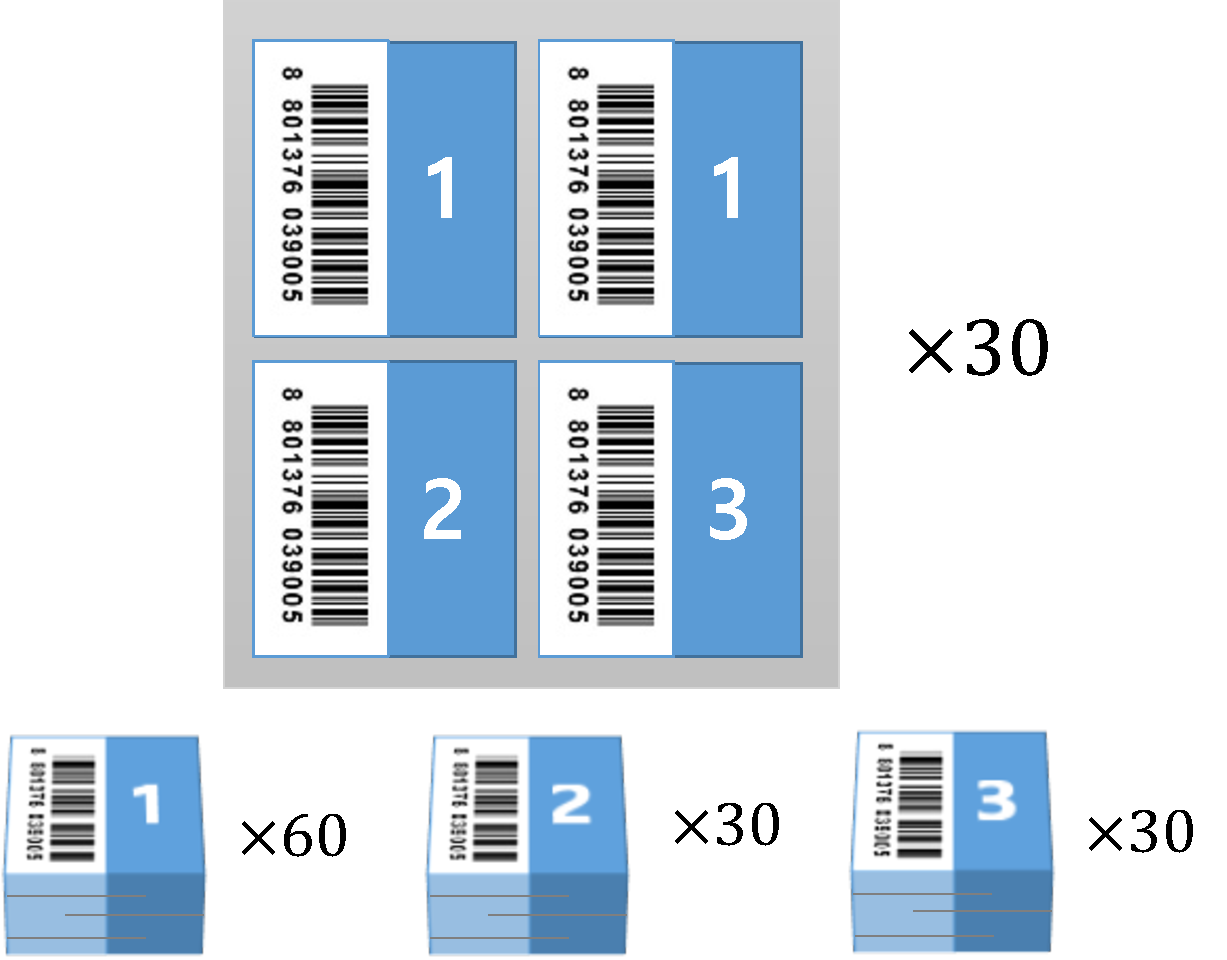
\includegraphics[width=4cm]{ex12.pdf}
		\caption{}
		\label{fig:ex12}       % Give a unique label
	\end{figure}
\end{example}

\begin{example}
	Assume that $I=\{1,2\}$, and ${\bf b}=(50,20)$.
	
	We consider $\pi = \{\{1,2\}\}$ is a partition for ${\bf b}$. Since $k = 4$, 
	the matrix $A = (\begin{array}{cc}2 & 2\end{array})$, and the printing number (\ref{eq:NumPlate}) is 
	\begin{equation}
	\left\lceil \max\left\{ \left. \frac{b_{i}}{A_{P,i}} \right| i \in P \right\} \right\rceil = \left\lceil \max \left\{ \frac{50}{2}, \frac{20}{2} \right\} \right\rceil = 25.
	\end{equation}
	The total number of Loss $E_{A,{\bf b}}$ is 30 (see Figure \ref{fig:ex21}).
	
	\begin{figure}[h!]
		\centering
		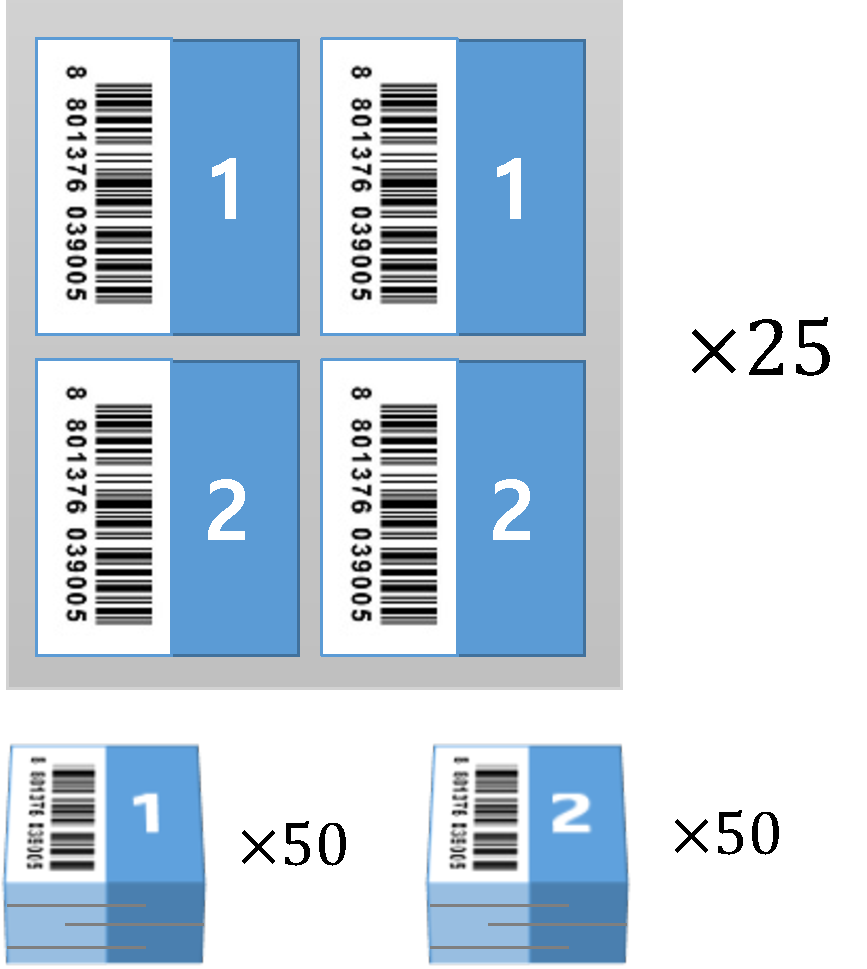
\includegraphics[width=3.5cm]{ex21.pdf}
		\caption{}
		\label{fig:ex21}       % Give a unique label
	\end{figure}
	
	For the same partition $\pi$, the matrix $A = (\begin{array}{cc}3 & 1\end{array})$ can be considered. In this case, the printing number (\ref{eq:NumPlate}) is 
	\begin{equation}
	\left\lceil \max\left\{ \left. \frac{b_{i}}{A_{P,i}} \right| i \in P \right\} \right\rceil = \left\lceil \max \left\{ \frac{50}{3}, \frac{20}{1} \right\} \right\rceil = 20.
	\end{equation}
	and the total number of Loss $E_{A,{\bf b}}$ is 10 (see Figure \ref{fig:ex22}).
	The array shown in Figure \ref{fig:ex22} is more efficient because its number of plate is the same but fewer losses occur.
	\begin{figure}[h!]
		\centering
		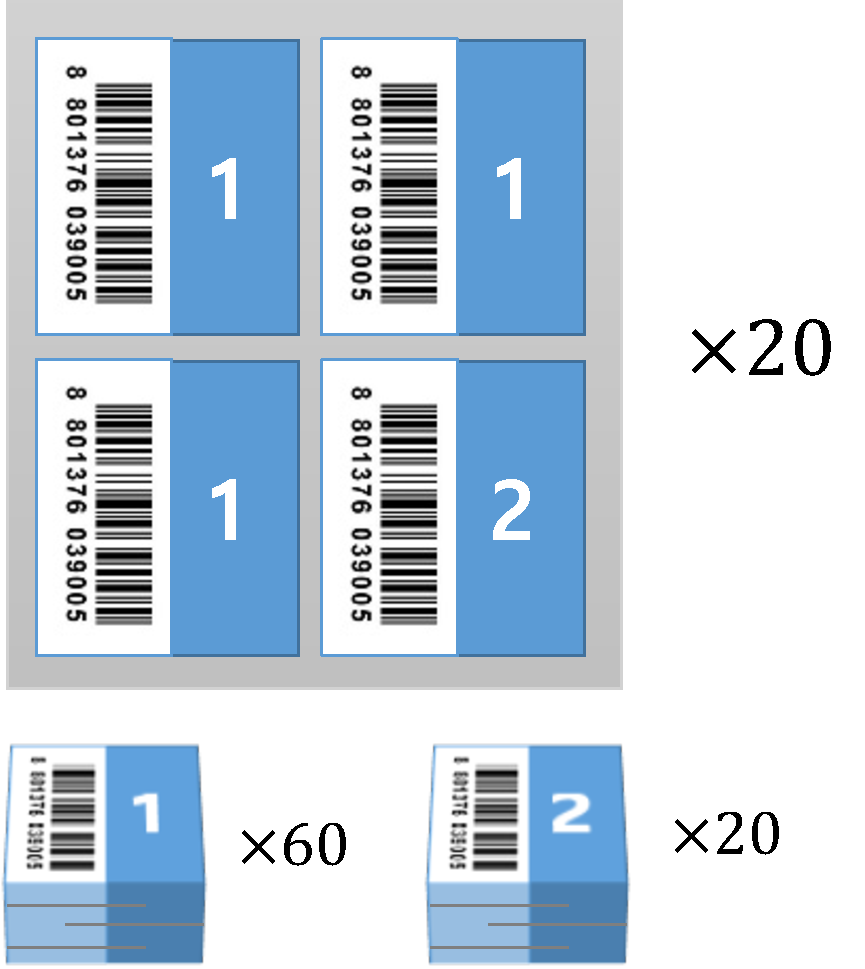
\includegraphics[width=3.5cm]{ex22.pdf}
		\caption{}
		\label{fig:ex22}       % Give a unique label
	\end{figure}
\end{example}


If there are so many products and also large order-quantity, it requires a lot of iteration. Now, we consider real problem of World Komax. In this case, $k=18$, $\alpha=300$, $\beta=1$. Table ~\ref{Tab:1} is an actual sorting report of an order from World Komax.

\begin{table}[h!]
	\centering
	\caption{the sorting report of World Komax}
	\begin{tabular}{ c|c|c|c|c|c|c } 
		\hline
		Plate&product&order-quantity&psc&printing-number&production&Loss\\
		\hline
		\multirow{5}*{1}
		&$1$&59&2&\multirow{5}*{32}&64&5\\
		\cline{2-4}
		\cline{6-7}
		&$2$&156&5&&160&4\\
		\cline{2-4}
		\cline{6-7}
		&$3$&9&1&&32&23\\
		\cline{2-4}
		\cline{6-7}
		&$4$&162&6&&192&30\\
		\cline{2-4}
		\cline{6-7}
		&$5$&102&4&&128&26\\
		
		\hline
		\multirow{5}*{2}
		&$6$&1059&5&\multirow{5}*{228}&1140&81\\
		\cline{2-4}
		\cline{6-7}
		&$7$&886&4&&912&26\\
		\cline{2-4}
		\cline{6-7}
		&$8$&228&1&&228&0\\
		\cline{2-4}
		\cline{6-7}
		&$9$&832&4&&912&80\\
		\cline{2-4}
		\cline{6-7}
		&$10$&862&4&&912&50\\
		
		\hline
		\multirow{4}*{3}
		&$11$&532&4&\multirow{4}*{133}&532&0\\
		\cline{2-4}
		\cline{6-7}
		&$12$&532&5&&665&133\\
		\cline{2-4}
		\cline{6-7}
		&$13$&482&4&&532&50\\
		\cline{2-4}
		\cline{6-7}
		&$14$&582&5&&665&103\\
		\hline
	\end{tabular}
	\label{Tab:1}	
\end{table}

As we can see from Table \ref{Tab:1}, there are $14$ products and the largest order-quantity is $1059$. It uses $3$ plates and total Loss is $611$. Total cost is $1511$.
\begin{example}
We obtain another partition of the sorting report using our algorithms. Table \ref{Tab:2} shows this result.
%Table \ref{Tab:2} shows the result calculated by our algorithm.

\begin{table}[h!]
	\centering
	\caption{the result of our algorithm}
	\begin{tabular}{ c|c|c|c|c|c|c } 
		\hline
		Plate&product&order-quantity&psc&printing-number&production&Loss\\
		\hline
		\multirow{6}*{1}
		&$7$&886&5&\multirow{6}*{178}&890&4\\
		\cline{2-4}
		\cline{6-7}
		&$10$&862&5&&890&28\\
		\cline{2-4}
		\cline{6-7}
		&$11$&532&3&&534&2\\
		\cline{2-4}
		\cline{6-7}
		&$12$&532&3&&534&2\\
		\cline{2-4}
		\cline{6-7}
		&$4$&162&1&&178&16\\
		\cline{2-4}
		\cline{6-7}
		&$2$&156&1&&178&22\\
		
		\hline
		\multirow{5}*{2}
		&$6$&1059&9&\multirow{5}*{118}&1062&3\\
		\cline{2-4}
		\cline{6-7}
		&$14$&562&5&&590&28\\
		\cline{2-4}
		\cline{6-7}
		&$8$&228&2&&236&8\\
		\cline{2-4}
		\cline{6-7}
		&$5$&102&1&&118&16\\
		\cline{2-4}
		\cline{6-7}
		&$1$&59&1&&118&59\\
		
		
		\hline
		\multirow{2}*{3}
		&$9$&832&11&\multirow{2}*{76}&836&4\\
		\cline{2-4}
		\cline{6-7}
		&$13$&482&7&&532&50\\
		
		\hline
		4&$3$&9&18&1&18&9\\
		\hline
	\end{tabular}
\label{Tab:2}	
  \end{table}

\noindent	
The matrix $A$ can be found as follows.
\begin{equation*}
\begin{array}{rc}
&\text{column index}\\
A\,\,=&
\begin{blockarray}{cccccccccccccc}
7 & 10 & 11 & 12 & 4 & 2 & 6 & 14 & 8 & 5 & 1 & 9 & 13 & 3\\
&&&&&&&&&&&&&\\
\begin{block}{(cccccccccccccc)}
5 & 5 & 3 & 3 & 1 & 1 & 0 & 0 & 0 & 0 & 0 & 0 & 0 & 0 \\
0 & 0 & 0 & 0 & 0 & 0 & 9 & 5 & 2 & 1 & 1 & 0 & 0 & 0 \\
0 & 0 & 0 & 0 & 0 & 0 & 0 & 0 & 0 & 0 & 0 & 11& 7 & 0 \\
0 & 0 & 0 & 0 & 0 & 0 & 0 & 0 & 0 & 0 & 0 & 0 & 0 & 18\\
\end{block}
\end{blockarray}
\end{array}
\end{equation*}
\noindent
The total Loss $E_{A,b}$ is $251$. So, total cost is $\alpha|\pi|+\beta E_{A,b}=300 \times 5+1 \times 251 =1451$. We use one more Plate, but the total cost is reduced by $60$.
%	As a result, we used the same number of plates, but because of less loss, our algorithm has less total cost.
	

	
\end{example}



\section{Result}\label{sec:Result}

Each sorting report includes the number of losses corresponding to one plate. 
Using this, the total cost can be calculated by replacing each plate with loss. 
We used 82 sorting report samples.
The total cost was reduced by from minimum -6.85\%(sample no. 15) to maximum 27.5\%(sample no. 74) (see Figure \ref{fig:Comparing}).

\begin{figure}[h!]
	\centering
%	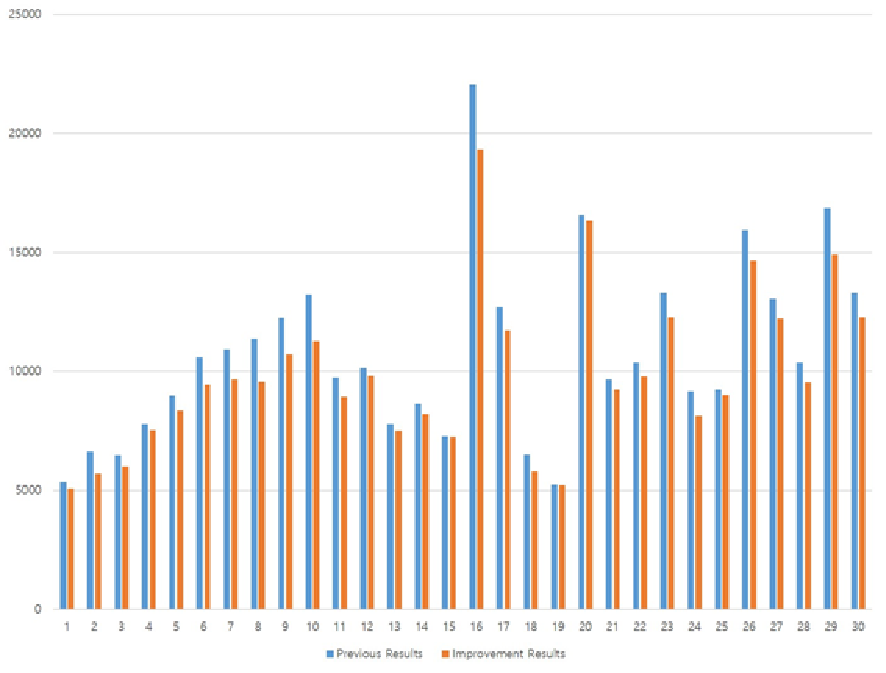
\includegraphics[width=\linewidth]{Comparing.pdf}
	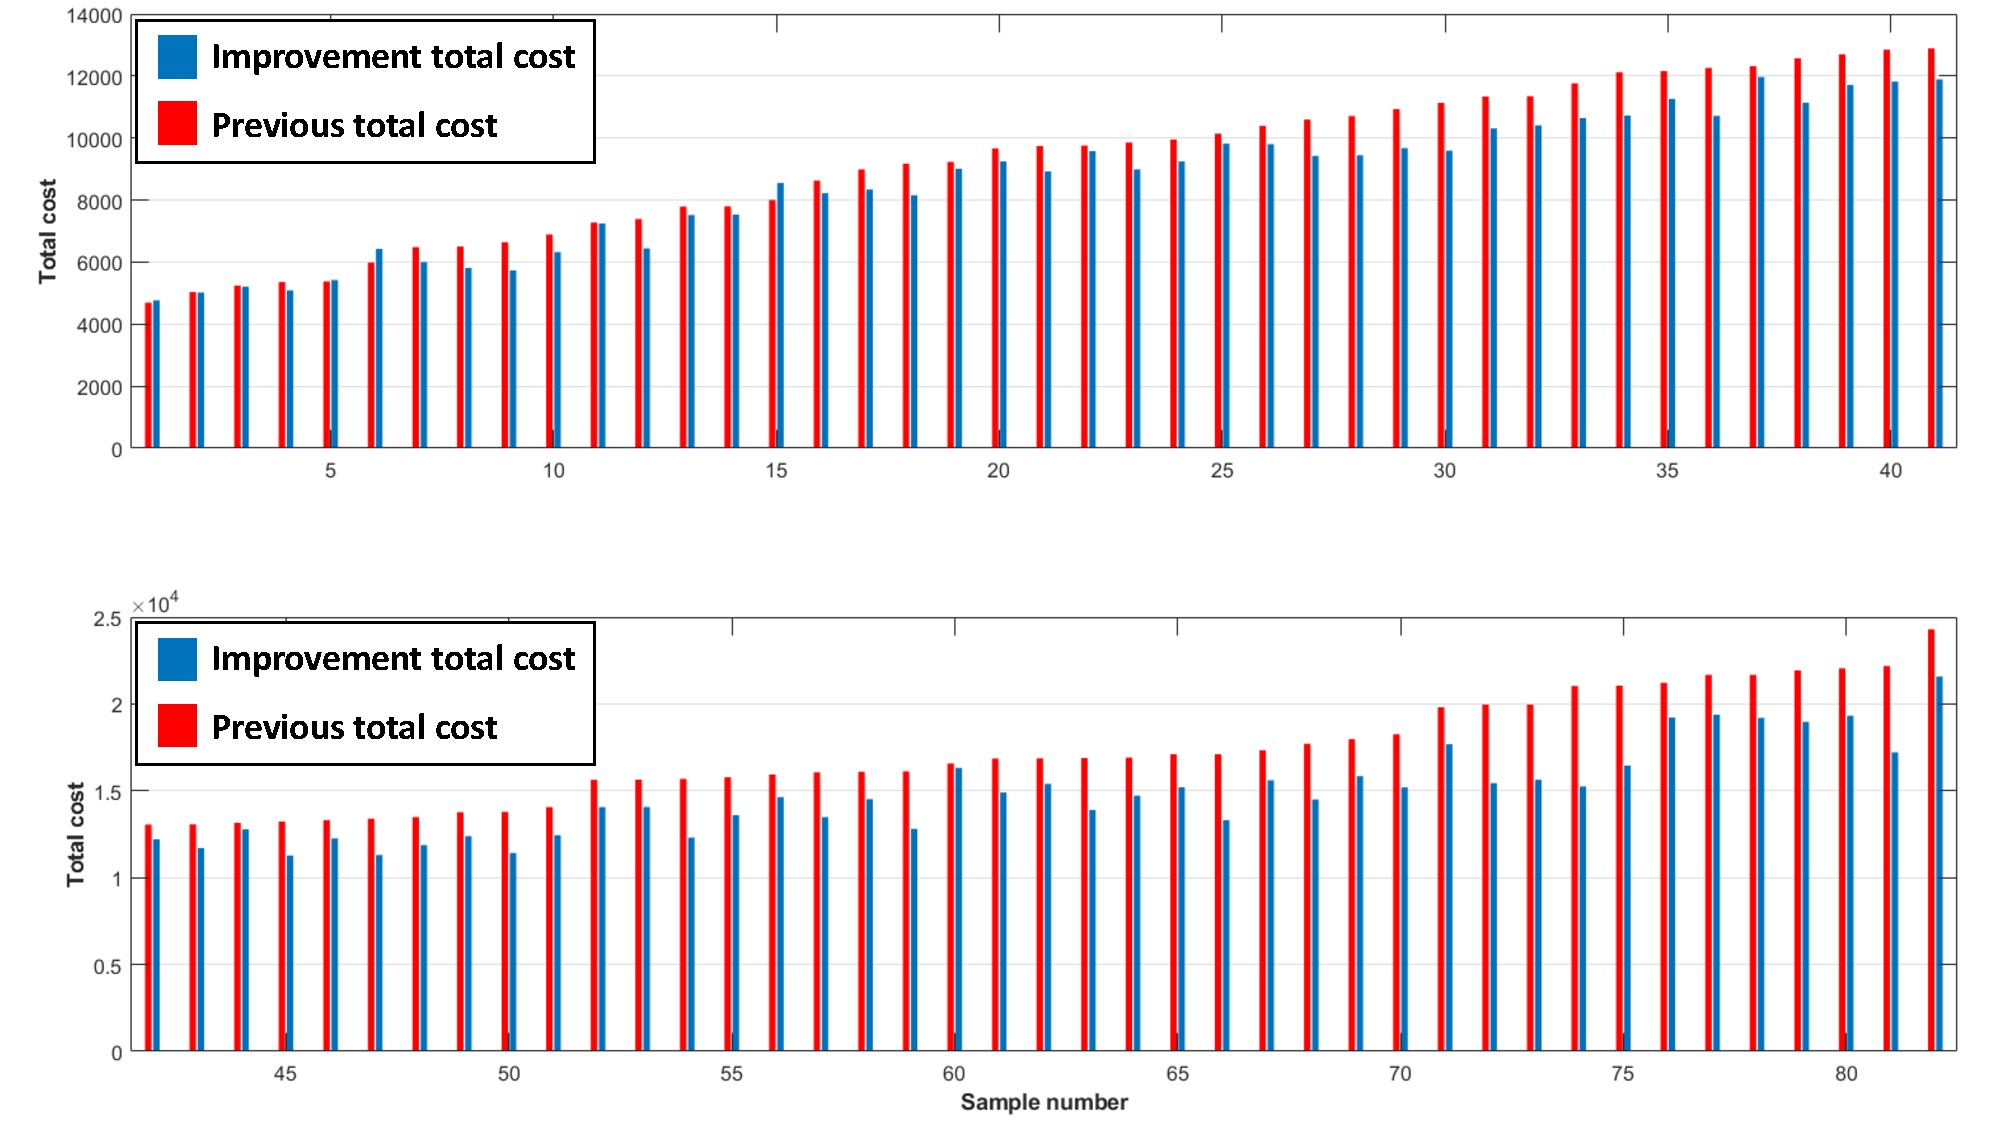
\includegraphics[width=11cm]{Graph_2.pdf}
	\caption{Comparing the Results}
	\label{fig:Comparing}       % Give a unique label
\end{figure}

We used the {\it paired t-test}\cite{Rice} to verify the efficiency of the algorithm. The pared t-test is one of the two sample t-test, and it is a test that verifies whether the two groups are different. The two populations are as follows.

\begin{enumerate}[$\bullet$]
	\item population1: total cost before applying the algorithm
	\item population2: total cost after applying the algorithm
	\item sample1: sample of 82 items from population1
	\item sample2: sample of 82 items from population2
\end{enumerate}

In order to proceed with the two-sample t-test, the two groups have to satisfy the normality and homoscedasticity. We choose $82$ sample data from the two populations, which can be satisfied the normality by the {\it central limit theorem} \cite{Durrett}.
In addition, we identified the homoscedasticity of the two samples through the {\it var.test} of R. 
R is a programming language and free software environment for statistical computing and graphic. % supported by the R Foundation for Statistical Computing. 
%The R language is widely used among statisticians and data miners for developing statistical software and data analysis.



The null hypothesis $(H_{0})$ of var.test is that `the variances of the two groups are equal', and the alternative hypothesis $(H_{1})$ is that `the variances of the two groups are different'. 
If the $p$-value is below the significance level, the null hypothesis $(H_{0})$ will be rejected and if the $p$-value is not lower than the significance level, the alternative hypothesis $(H_{1})$ will be rejected.  The result of var.test with the significance level to 0.05 is as follows (see Figure \ref{fig:vartest}).

\begin{figure}[h!]
	\centering
	\fbox{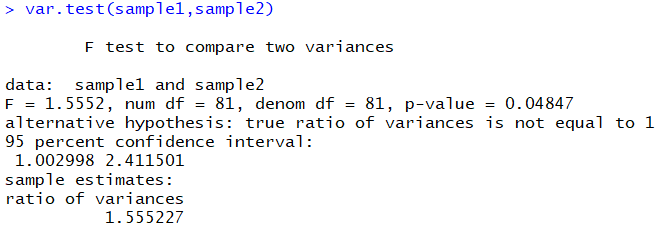
\includegraphics[width=8cm]{vartest.png}}
	\caption{var.test of R}
	\label{fig:vartest}       % Give a unique label
\end{figure}

Since the $p$-value is not lower than the significance level(0.05), the alternative hypothesis $(H_{1})$ is rejected and the null hypothesis $(H_{0})$ is accepted. 
We say that the variances of the two groups can be equal.

Since the two groups satisfy normality and homoscedasticity, we verified whether the difference between the two groups is significant through paired t-test. In this test, the null hypothesis $(H_{0})$ is `the total cost will be the same after applying the algorithm.' and the alternative hypothesis $(H_{1})$ is `the total cost will be reduced after applying algorithm.' The result of the paired t-test with the significance level to 0.05 is as follows (see Figure \ref{fig:ttest}).

\begin{figure}[h!]
	\centering
	\fbox{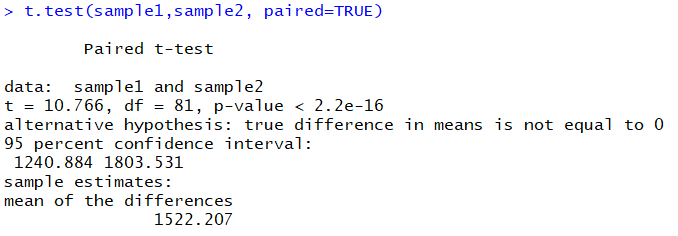
\includegraphics[width=8cm]{ttest.png}}
	\caption{t.test of R}
	\label{fig:ttest}       % Give a unique label
\end{figure}

Since the $p$-value is below the significance level(0.05), the null hypothesis $(H_{0})$ is rejected and the alternative hypothesis $(H_{1})$ is accepted. We say that the difference between the two groups can be significant.

Finally, we check the efficiency over the number of products which is the size of $I$(cf. Section \ref{sec:Modeling}).
We see that the efficiency increases as the number of products increases in Figure \ref{fig:LinearFitting}.
For each 82 samples, we calculated the efficiency as the follow formula.
\begin{equation}
	\textrm{Efficiency} = \left[1-\frac{\textrm{Improvement~Total~Cost}}{\textrm{Previous~Total~Cost}}\right]\times 100
\end{equation}
The result of the linear fitting shows that the efficiency and the number of products have a positive correlation.
Thus, we see that the improved algorithms have better results in many number of products.
This suggests that the algorithm fits well into small quantity batch productions.


\begin{figure}[h!]
	\centering
	%	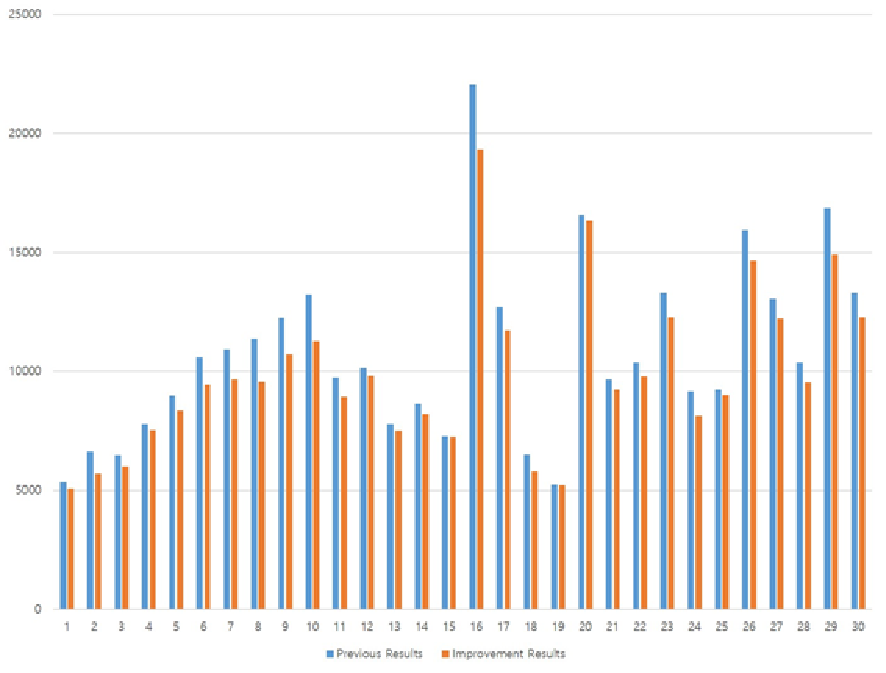
\includegraphics[width=\linewidth]{Comparing.pdf}
	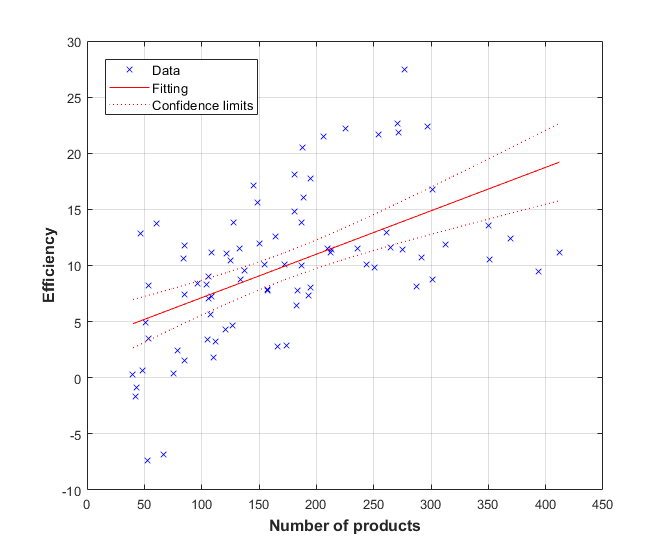
\includegraphics[width=7.5cm]{Graph_3.png}
	\caption{The linear fitting for the efficiency over the number of products}
	\label{fig:LinearFitting}       % Give a unique label
\end{figure}


{\bf Notice.} Please note that the detailed idea of the algorithm cannot be described for confidentiality of the company.

~\\
\indent{{\bf Acknowledgements.} This work was supported by the National Research Foundation of Korea (NRF)
grant funded by the Korean Government (MSIP) (NRF-2017R1A5A1015722, NRF-2018R1D1A1B07048197). 
%The authors thank the anonymous referees for providing very useful suggestions for improving this paper.
The authors extend thanks to Professor Hyun-Min Kim and Professor Sang-il Kim of Pusan National University who provided many support and advises for the writing of this paper.}

\bibliographystyle{plain}
\bibliography{mybibfile}

\end{document}
% end of file template.tex

g